\documentclass{article}

\usepackage{parskip}
\usepackage{amsmath}
\usepackage{amssymb}
\usepackage{minted}
\usepackage{graphicx}
\usepackage{caption}
\usepackage{subcaption}
\usepackage[final]{pdfpages}
\usepackage[letterpaper,top=2cm,bottom=2cm,left=2cm,right=2cm,marginparwidth=1.75cm]{geometry}
\usepackage[backend=biber,sorting=ynt,doi=false,url=true,]{biblatex}
\usepackage[hidelinks]{hyperref}
\DeclareFieldFormat{doi/url-link}{#1}

\addbibresource{ref.bib}
\graphicspath{ {./images/} }

\begin{document}

\title{\textbf{CSC 579 Project Bi-Weekly Update 2 \protect\\ QoE Improvements For Adaptive Video Streaming Over SDN-Enabled Networks}}

\author{Jinwei Zhao, Fatima Amri}

\date{\today}

\maketitle

\section{Bi-weekly Update 2}
Over the past two weeks, we have been working on different parts of the project.
Since the authors of \cite{bhat_network_2017} released their code on GitHub, Jinwei has been trying to deploy their code and reproduce their results on CloudLab. In the meantime, Fatima has been understanding the mathematical details of \cite{mu_scalable_2016} because we will have to implement this paper on our own. The current progress of deploying SABR code \cite{bhat_network_2017} on CloudLab is introduced in Section 2. In Section 3, we include some details of our understanding of the mathematical details of \cite{mu_scalable_2016}. 

\section{Deploying SABR code on CloudLab, by Jinwei}

\cite{bhat_network_2017} released their code on GitHub five years ago(\url{https://github.com/dbhat/SABR}). The original code was based on Python 2. Since Python 2 has been deprecated since January 1, 2020, there is a fork on GitHub made available by GitHub user mwhicks-dev(\url{https://github.com/mwhicks-dev/SABR}), that migrated the original code to Python 3. Our course project is based on mwhicks-dev's fork, which can be found here: \url{https://github.com/CSc579s22}. 

\subsection{Code structure}

In order to deploy and reproduce SABR on CloudLab, there are four different code repositories involved in total. 

\begin{enumerate}
    \item SABR(\url{https://github.com/CSc579s22/SABR}): This is the \textit{main} repository containing the original work done by \cite{bhat_network_2017}. 
    \item cloudlab\_SABR(\url{https://github.com/CSc579s22/cloudlab_SABR}): This repository contains CloudLab related code from \cite{bhat_network_2017}, e.g., server topology, bootstrap scripts. 
    \item AStream(\url{https://github.com/CSc579s22/AStream}): AStream is a Python based emulated video player to evaluate the performance of the DASH bitrate adaptation algorithms.
    \item SDN-OpenNetMon(\url{https://github.com/CSc579s22/SDN-OpenNetMon}): OpenNetMon offers an accurate and precise OpenFlow Monitoring POX module by \cite{openmon}.
\end{enumerate}

\subsection{Server Topology}

The server topology described in \cite{bhat_network_2017} is shown in Figure \ref{fig:sabr_og_topo}. Based on the server topology file in the code(\url{https://github.com/dbhat/cloudlab_SABR/blob/master/profile.rspec}), we managed to illustrate the actual server topology in Figure \ref{fig:sabr_code_og}.

\begin{figure}[!tbp]
  \begin{subfigure}[b]{0.45\textwidth}
    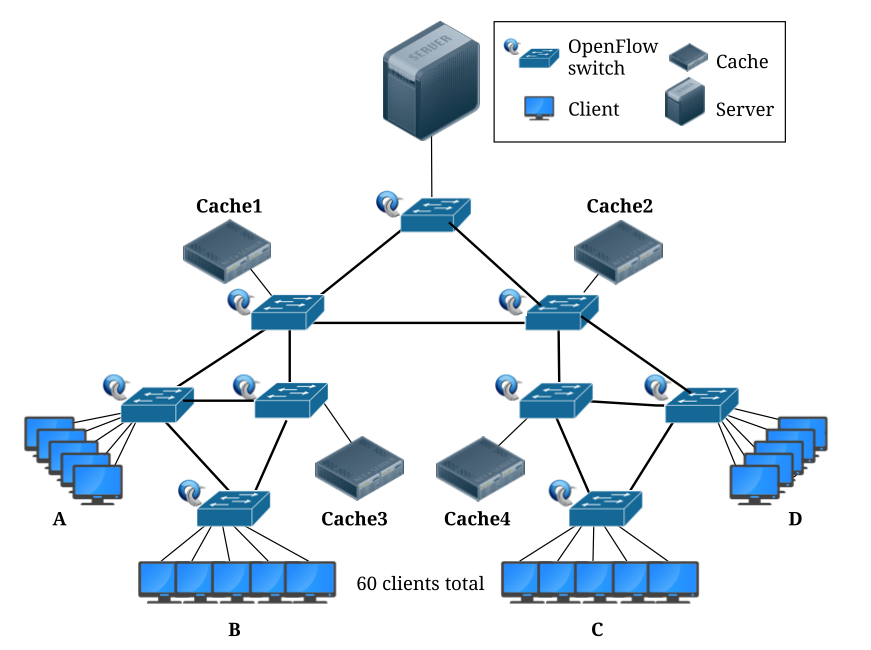
\includegraphics[width=\textwidth]{images/sabr_og_topo.png}
    \caption{The server topology described in \cite{bhat_network_2017}}
    \label{fig:sabr_og_topo}
  \end{subfigure}
  \hfill
  \begin{subfigure}[b]{0.45\textwidth}
    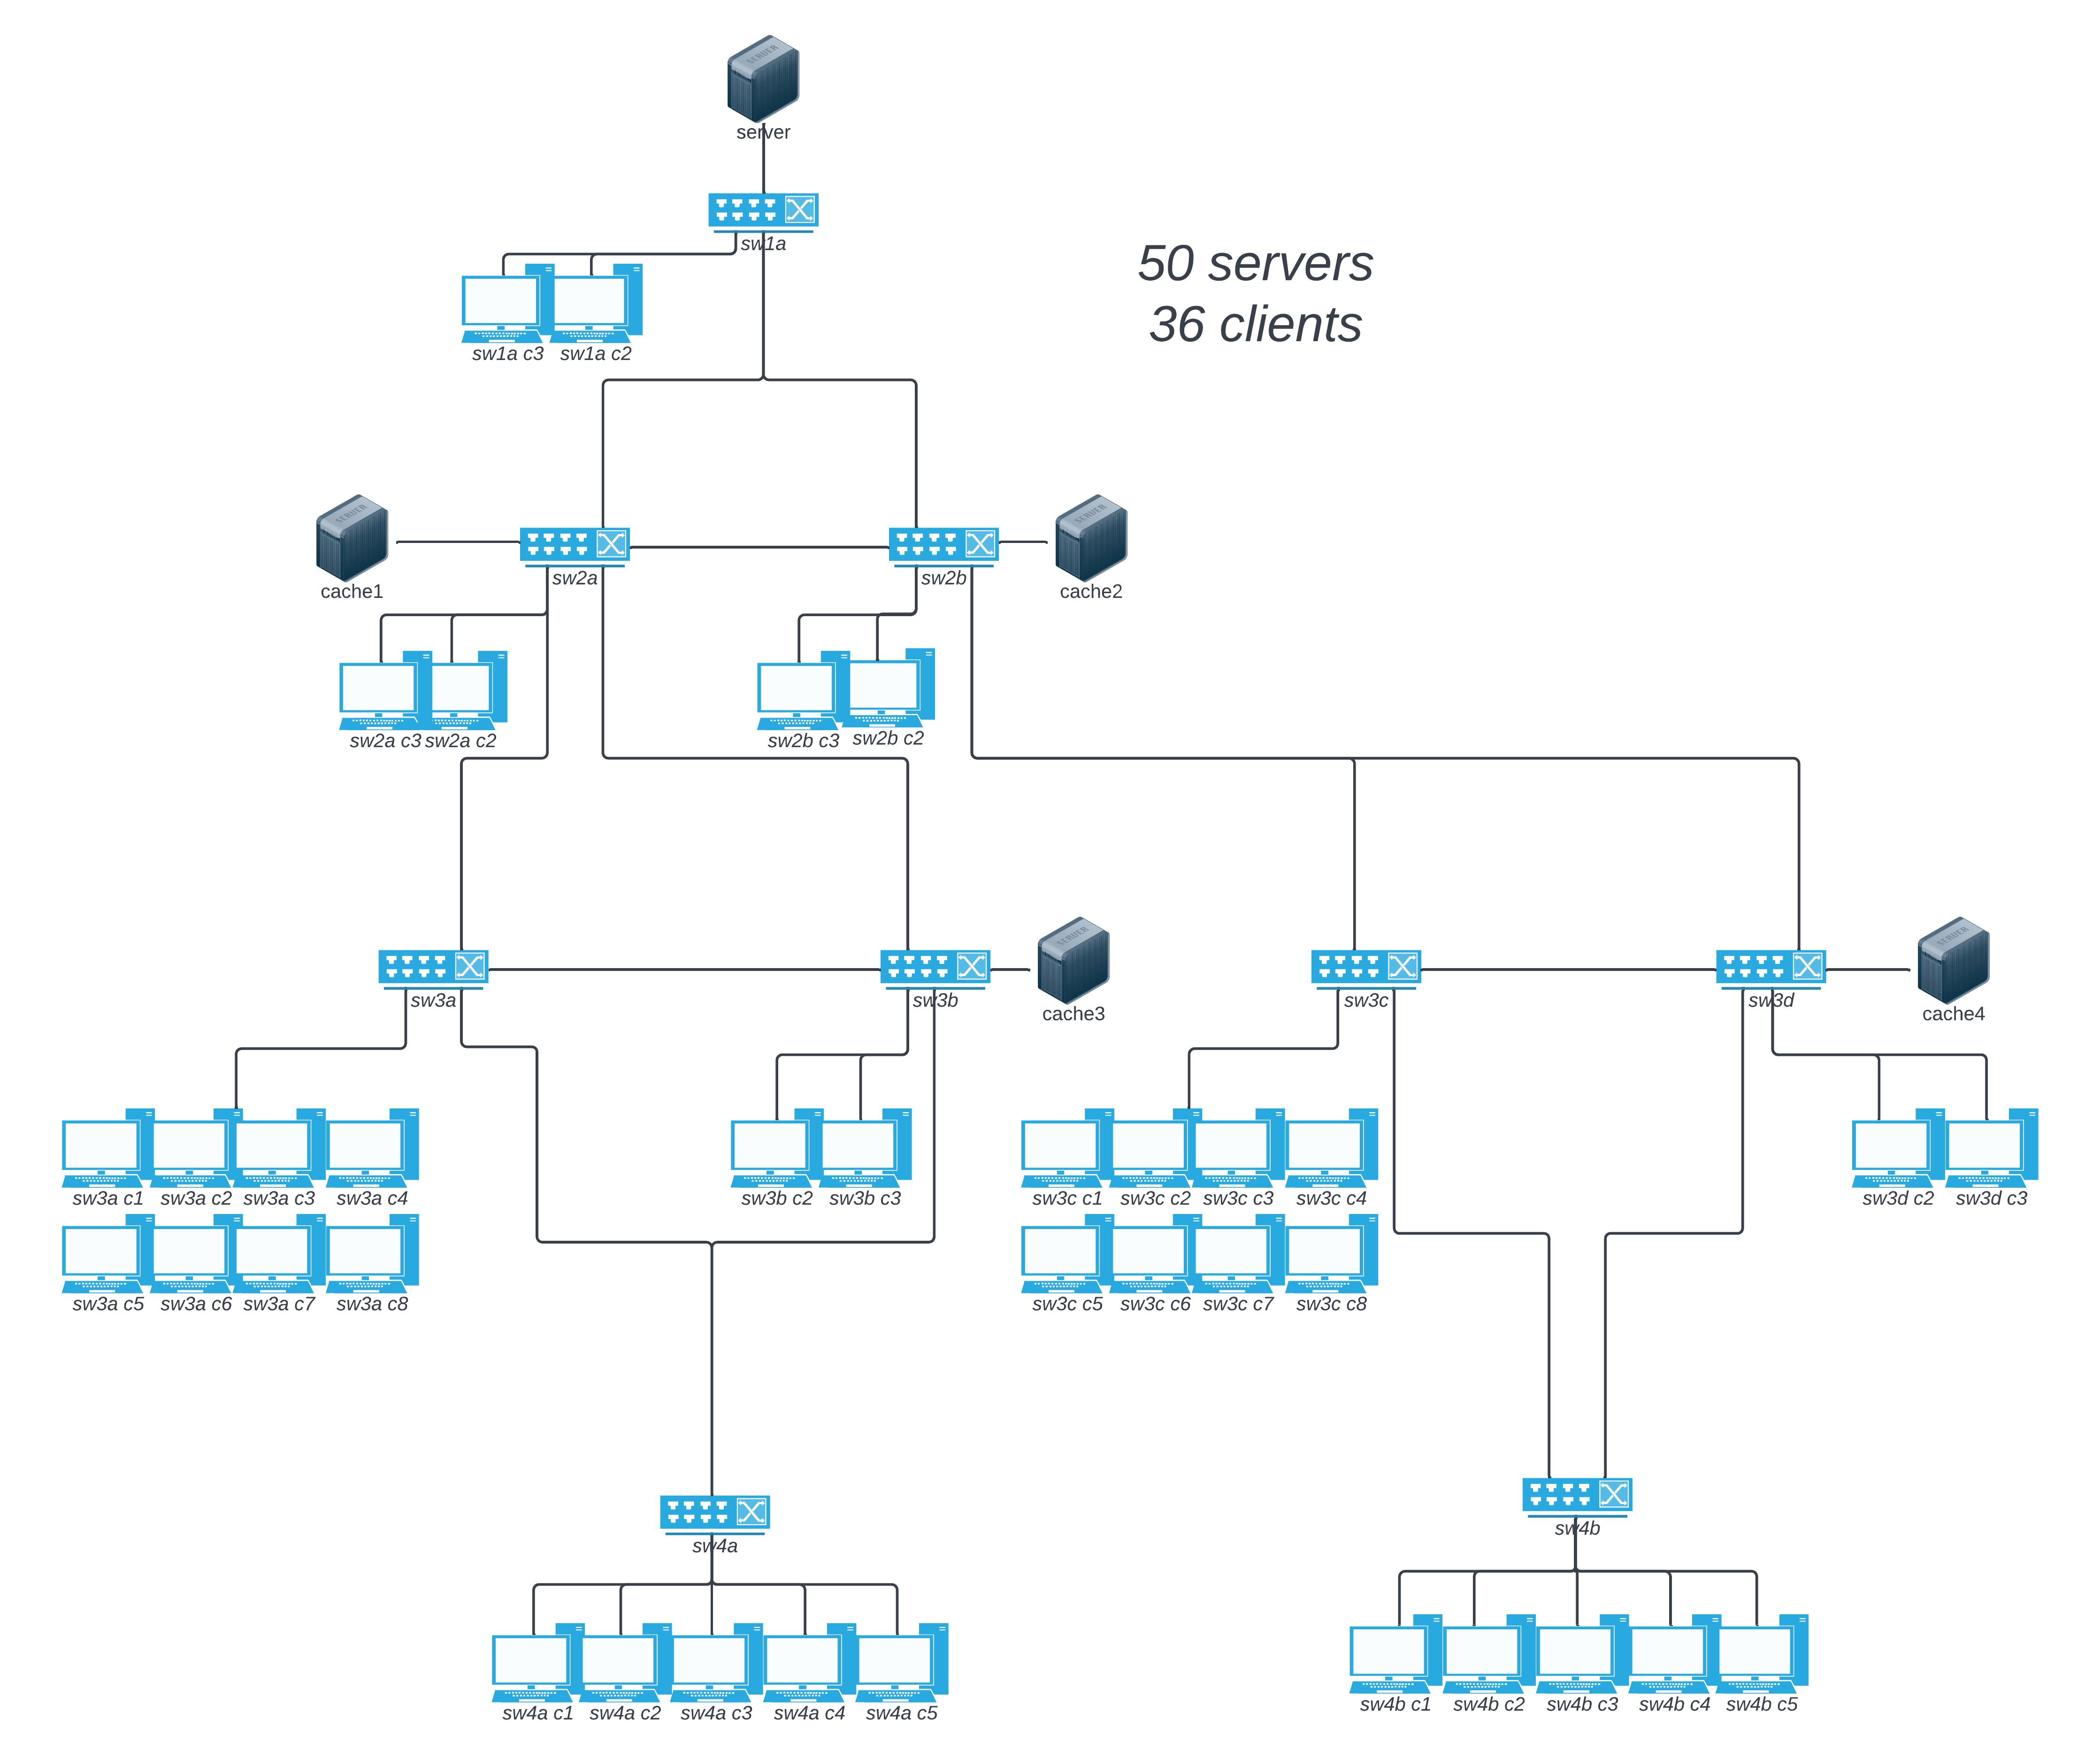
\includegraphics[width=\textwidth]{images/SABR_code_og.png}
    \caption{The server topology provided in code}
    \label{fig:sabr_code_og}
  \end{subfigure}
  \caption{Server topologies}
  \label{fig:server}
\end{figure}

\subsection{Server provisioning on CloudLab}

The switches in Figure \ref{fig:server} are actually software switches implemented by Open vSwitch(OVS). The authors used a total of 50 XEN virtual machines on CloudLab for both the switches and clients. At first, we followed their strategy and used XEN virtual machines as well. But among our attempts, there was always a possibility that several XEN virtual machines failed to initialize and boot, with their status labelled as \textit{TBFAILED}. 

% \begin{figure}
% \centering
% 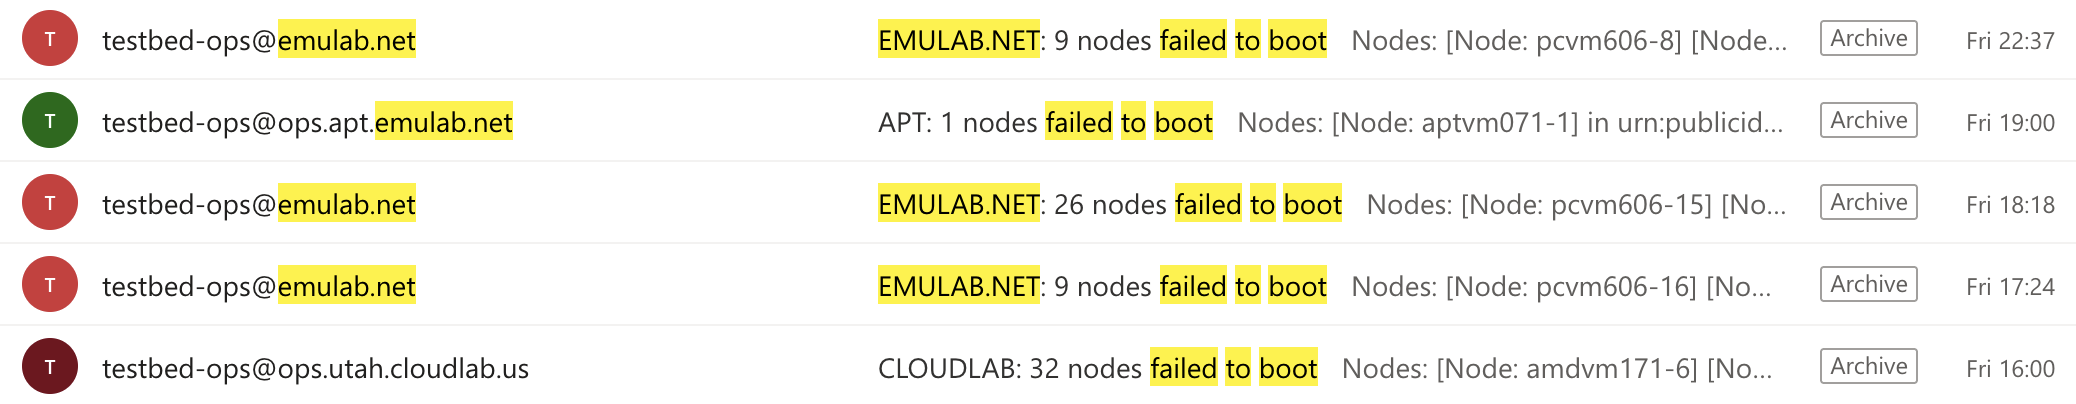
\includegraphics[width=\textwidth]{images/tbfailed.png}
% \caption{XEN vms failed to initialize and boot}
% \label{fig:tbfailed}
% \end{figure}

After several failed attempts, we decided to go to \textbf{Hybrid} mode. Since we have to use multiple Ethernet ports to connect to different clients on OVS switch nodes, i.e., different ports connected to the same bridge in OVS, we still have to use XEN virtual machines for OVS switch nodes. But for the streaming server, cache nodes and streaming clients, we use bare metal servers(Bare metal servers are easier to provision and schedule than XEN virtual machines on CloudLab). And we also reduced the total number of streaming clients to 18 in order to reduce the resource consumption on CloudLab. The server topology that we use to provision servers on CloudLab is shown in Figure \ref{fig:our-topology}. 

\begin{figure}
\centering
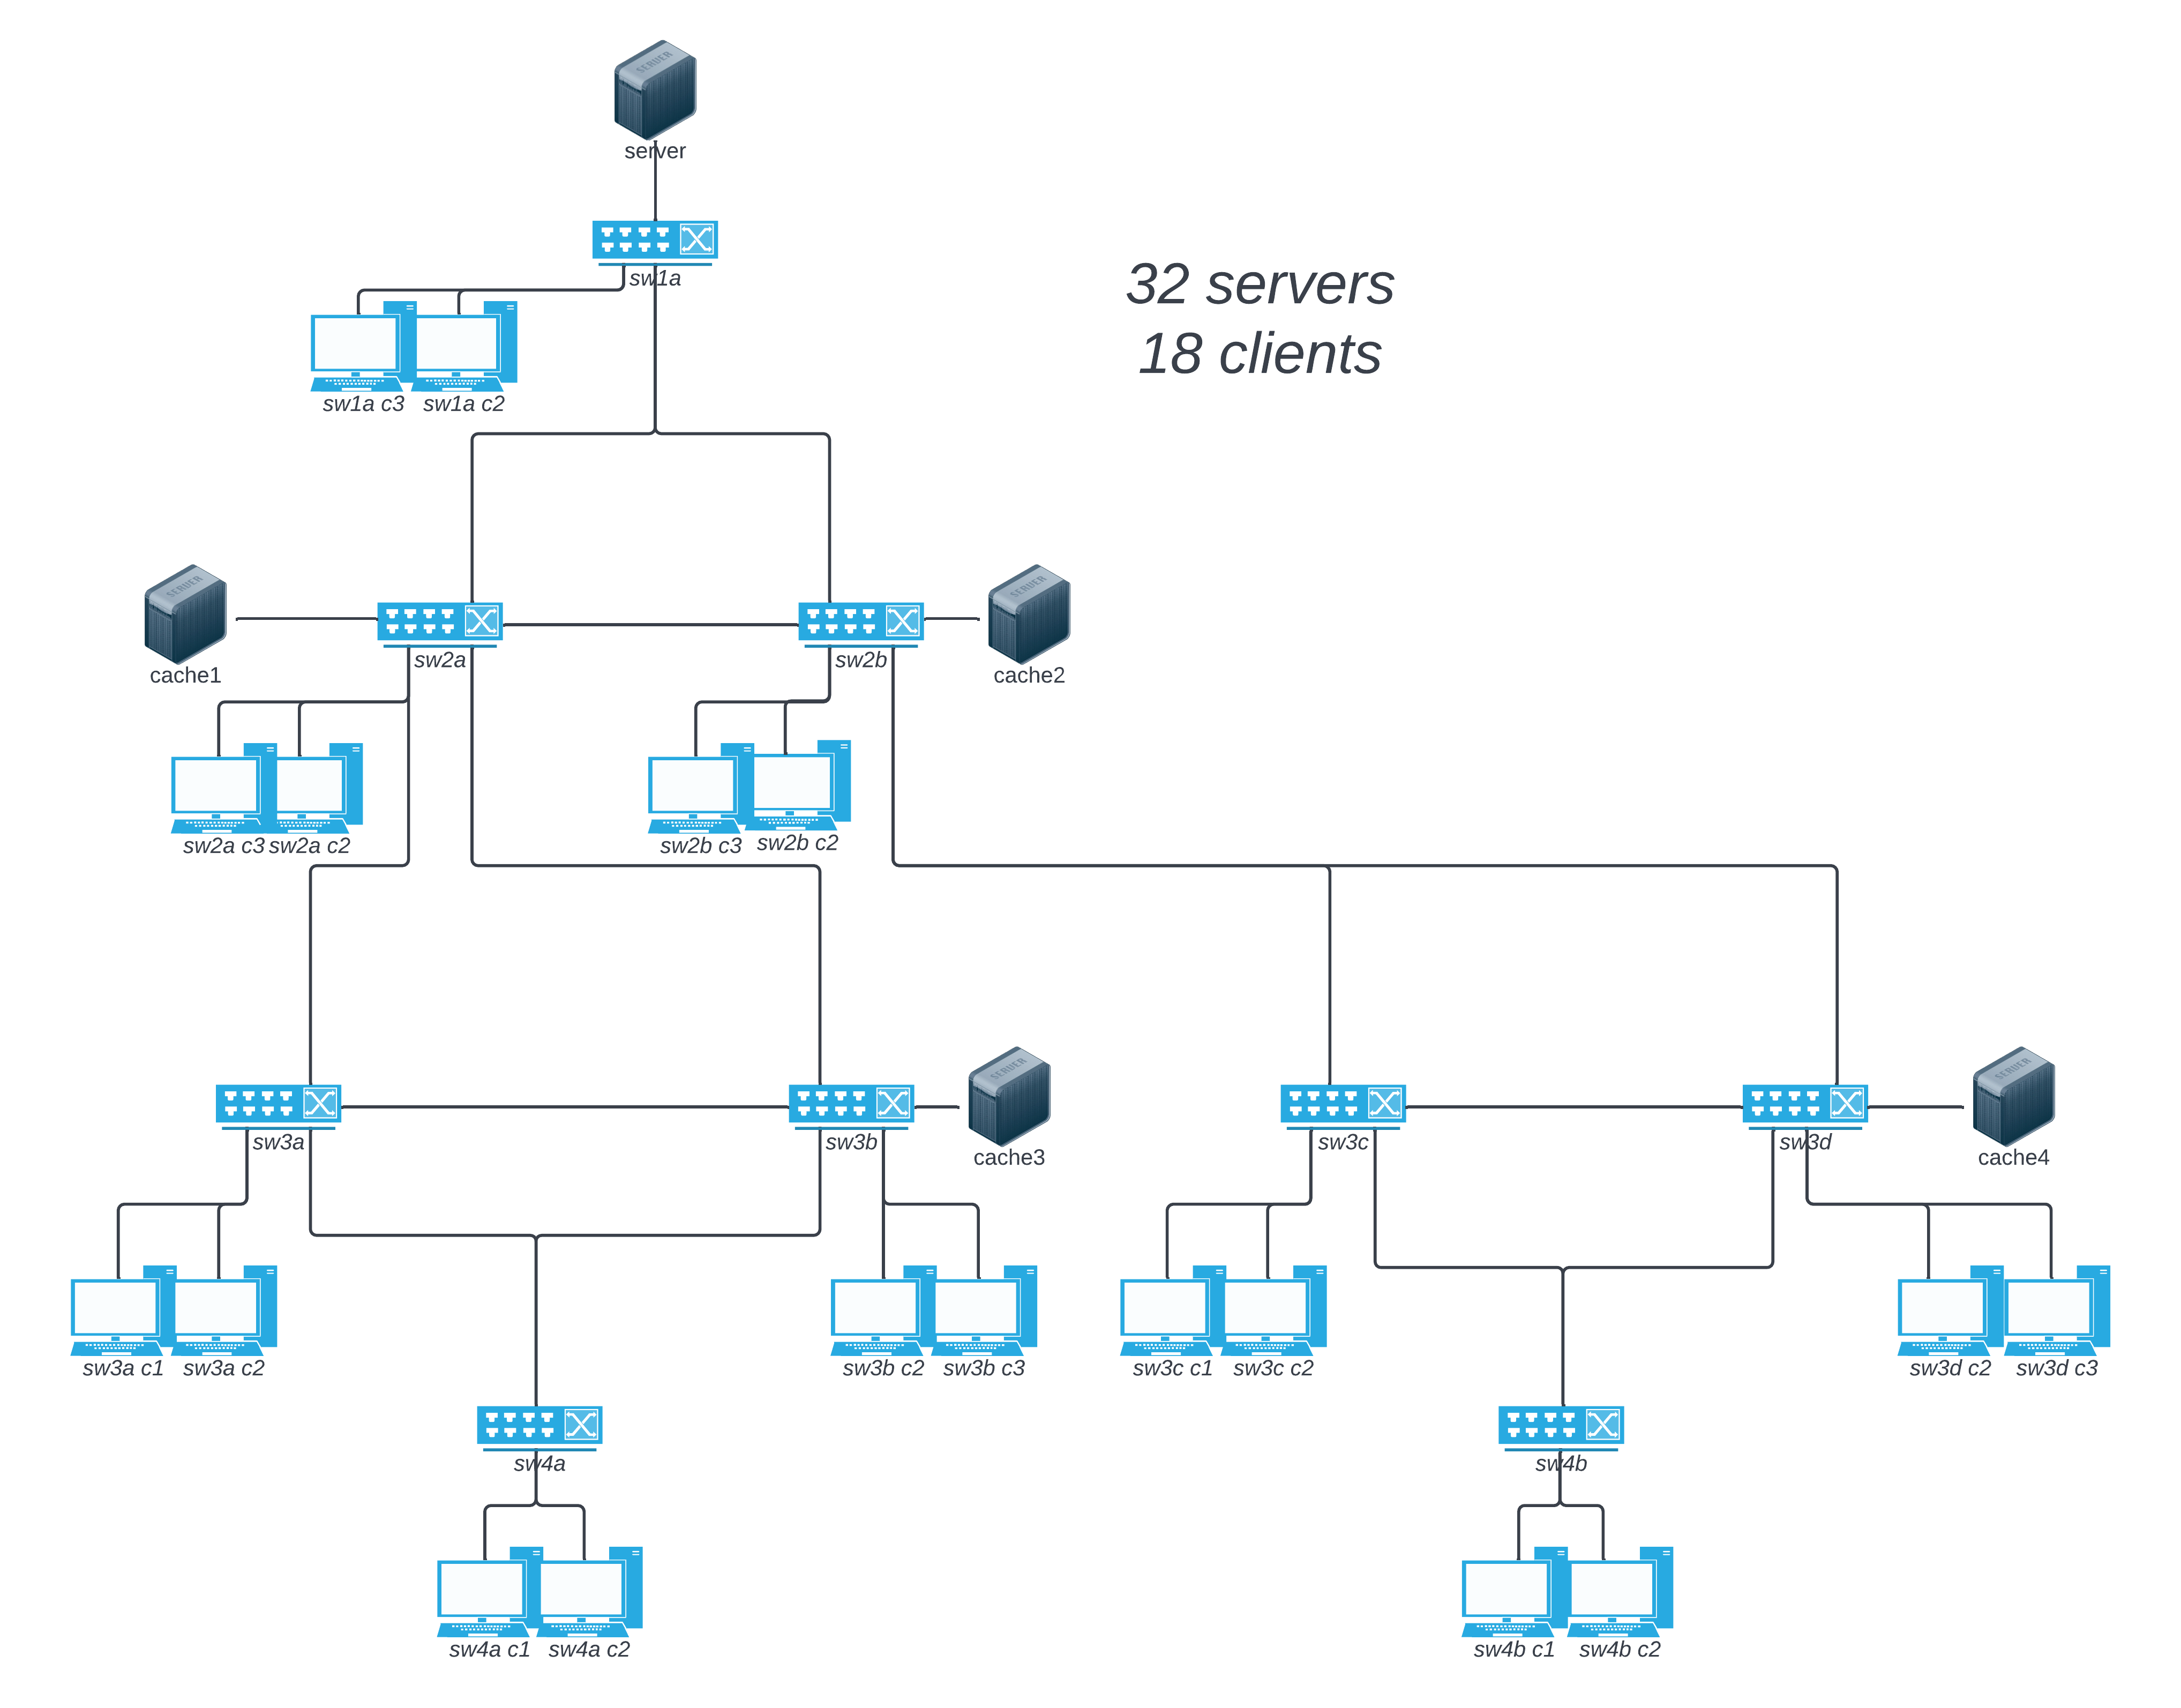
\includegraphics[width=0.5\textwidth]{images/SBAR Simple.png}
\caption{Our server topology}
\label{fig:our-topology}
\end{figure}

\subsection{Install dependencies for SABR}

Installing dependencies is straightforward. Following the steps in the README file of SABR project(\url{https://github.com/dbhat/SABR/blob/master/README.md}), here is a curated shell script of major steps we've done so far. An updated and complete version will be included in our fork of SABR repository(\url{https://github.com/CSc579s22/SABR}) by the end of the project. 

\subsubsection{Setup on streaming server}

\begin{minted}[breaklines]{bash}
cd /proj/QoESDN
git clone https://github.com/CSc579s22/SABR.git
git clone https://github.com/CSc579s22/cloudlab_SABR.git
git clone https://github.com/CSc579s22/AStream.git
git clone https://github.com/CSc579s22/SDN-OpenNetMon.git
cd SDN-OpenNetMon
git submodule update --init --recursive
mkdir -p pox/ext/opennetmon
git clone https://github.com/TUDelftNAS/SDN-OpenNetMon pox/ext/opennetmon

cd /tmp/

# install basic dependencies
sudo apt update && sudo apt install -y zsh mongodb vim screen apache2 build-essential libssl-dev libffi-dev htop
sudo systemctl enable mongodb apache2
sudo systemctl restart mongodb apache2

# install R
sudo apt update 
sudo apt install -y software-properties-common dirmngr
wget -qO- https://cloud.r-project.org/bin/linux/ubuntu/marutter_pubkey.asc | sudo tee -a /etc/apt/trusted.gpg.d/cran_ubuntu_key.asc
sudo add-apt-repository "deb https://cloud.r-project.org/bin/linux/ubuntu $(lsb_release -cs)-cran40/"
sudo apt install r-base -y

# install forecast package for R
# https://github.com/robjhyndman/forecast
sudo apt install -y libz-dev libssl-dev libxml2-dev libcurl4-openssl-dev gfortran libblas-dev liblapack-dev
sudo Rscript -e "install.packages('forecast', dependencies = TRUE)"

# install python3 and rpy2
sudo apt -y install python3 python3-dev python3-pip
sudo pip install rpy2\[all\] pymongo scapy scapy_http netifaces

# install python2 and pip2 for arima and opennetmon
sudo apt -y install python2 python2-dev 
wget https://bootstrap.pypa.io/pip/2.7/get-pip.py
sudo python2 get-pip.py
sudo pip install requests pymongo numpy scipy 
sudo apt install -y libreadline-dev libbz2-dev liblzma-dev libpcre2-dev

sudo pip install 'pandas<0.19' 'rpy2<2.9.0'

# prepare mpd file for streaming(this step seems problematic, we will investigate later)
cd /var/www/html
sudo wget -r --no-parent --reject \"index.html*\" http://www-itec.uni-klu.ac.at/ftp/datasets/DASHDataset2014/BigBuckBunny/2sec/
sudo cp /proj/QoESDN/cloudlab_SABR/server/BigBuckBunny_2s_mod* /var/www/html/www-itec.uni-klu.ac.at/ftp/datasets/DASHDataset2014/BigBuckBunny/2sec/
for i in `seq 1 50`;
do
        sudo mkdir /var/www/html/BigBuckBunny_2s_mod$i
        sudo ln -s /var/www/html/www-itec.uni-klu.ac.at/ /var/www/html/BigBuckBunny_2s_mod$i/www-itec.uni-klu.ac.at
done

cd /proj/QoESDN/cloudlab_SABR/server
python3 create_mpdinfo.py

# start opennetmon controller
cd /proj/QoESDN/SDN-OpenNetMon/pox
sudo ./pox.py openflow.of_01 --port=1234 log --file=opennetmon.log,w opennetmon.startup

# start ARIMA forecast
cp /proj/QoESDN/SABR/controllerSABR/arima.py /proj/QoESDN/SDN-OpenNetMon/pox/ext/
cd /proj/QoESDN/SDN-OpenNetMon/pox
sudo ./pox.py openflow.of_01 --port=1235 log --file=arima.log,w arima

# start listening requests for caching
cd /proj/QoESDN/cloudlab_SABR/server
sudo python3 http_capture.py

\end{minted}

\subsubsection{Setup on each OVS switch node}

\begin{minted}[breaklines]{bash}
# install openvswitch
sudo apt update
sudo apt install -y openvswitch-switch
sudo systemctl enable openvswitch-switch
sudo systemctl restart openvswitch-switch

# create ovs bridge
sudo ovs-vsctl add-br br0

# add ports to ovs bridge accordingly
sudo ovs-vsctl add-port br0 eth1

# set bridge controller to pox
sudo ovs-vsctl set-controller br0 tcp:<ip>:<port>
\end{minted}

\subsubsection{Setup on each streaming client}

\begin{minted}[breaklines]{bash}
sudo apt install -y python3 python3-dev python3-pip
sudo pip install urllib3 httplib2 pymongo netifaces requests numpy sortedcontainers
\end{minted}

\subsection{Progress and Issues}
So far, we've provisioned servers on CloudLab according to our topology, and installed software dependencies. The authors provided MPD files in cloudlab\_SABR repository(\url{https://github.com/dbhat/cloudlab_SABR/tree/master/server}), but the actual video files are missing. I managed to find the corresponding video files at \url{http://ftp.itec.aau.at/datasets/DASHDataset2014/BigBuckBunny/}. A script to download these video files to the streaming server is needed. 

The Astream client(\url{https://github.com/CSc579s22/AStream}) has problems parsing MPD files from (\url{https://github.com/dbhat/cloudlab_SABR/tree/master/server}). I will use the example MPD file available at \url{https://github.com/CSc579s22/AStream/tree/master/dist/sample_mpd} instead. 

\section{Mathematical details for \texorpdfstring{\cite{mu_scalable_2016}}, by Fatima}

As we mentioned in previous project updates, there are three fairness metrics that this paper has focused on: video quality, switching impact and cost efficiency. To this end, formulating the fairness for each of them is required. 

\textbf{Video Quality (VQ) Fairness}: In general, a HAS application chooses an optimal resolution for the playback device and dynamically selects a representation from the adaptation set according to the available bandwidth. It is proved in the paper that there is a non-linear relationship between bitrate and video quality as follows: 

\begin{equation}
Q_{resolution}=a \cdot r^b+c
\end{equation}

where $r$ is the video bitrate, $a,b$ and $c$ are constant (they are provided in Table 1 in the paper). A $Q$ of 1 is the maximum possible video quality. The above equation is also known as the generic QoE utility function ($U_{res}(r)$). They have rescaled the utility function, $U_{res}(r)$, so that the video quality reaches its maximum and close to 1 when the maximum representation is active. The $r^{MAX}$ is the maximum bitrate that network resources can provide. Therefore, we have:

\begin{equation}
U\prime_{r e s}(r)=\frac{U_{r e s}(r)}{U_{r e s}\left(r^{M A X}\right)}
\end{equation}

The VQ fairness between media streams is measured using Relative Standard Deviation (RSD) as follow. The intuition behind this is decreasing the video quality difference between different streams so that all streams have a good and same quality.

\begin{equation}
\begin{aligned}
\text{standard deviation} &=s_{V Q}=\operatorname{sqrt}\left(\frac{1}{M-1} \sum_{j=1}^{M}\left(Q_{j}-\bar{Q}\right)^{2}\right) \\
R S D &=\mathfrak{I}^{V Q}=\frac{100 \times s_{V Q}}{\bar{Q}}
\end{aligned}
\end{equation}

Low RSD means less difference in VQ of streams, so better user-level fairness. The maximum fairness is when $\mathfrak{J}^{V Q}$ reaches zero.

\textbf{Switching Impact (SI) Fairness}: Basically, HAS streams switch between different representations to adopt the available network resources. This switching can either improve the video quality or reduce it while resource is limited. The switching impact is influenced by two factors: the amplitude and the distribution of switching. The amplitude is determined by the perception of video quality changes between representations, and the intensity of quality changes can be formulated by $\Delta_{V Q}=|Q-Q\prime|$, where $Q\prime$ is the projected video quality after the representation switch.

The forgiveness effect is used for modeling the switching impact. Forgiveness effect captures the psychological observations that the impact of quality distortion degrades over time.

\begin{equation}
S I_{i}(t)=\left(\Delta_{V Q}\right) \cdot e^{-0.015\left(t-t_{i}\right)}
\end{equation}

Where $t_i$ is the time of the quality switch $i$. 
On the other hands, it is stated that 10\% of the initial switch impact as a residual influence that lasts for the user’s entire viewing session. So, the SI formulation can be rewrite as follows:

\begin{equation}
S I_{i}(t)=\max \left(\left(\Delta_{V Q}\right) \cdot e^{-0.015\left(t-t_{i}\right)}, 0.1 \Delta_{V Q}\right)
\end{equation}

Switching impact accounts for the frequency and distribution of changes over the playing time. And with help of SI, switching impact fairness function based on RSD is introduced:

\begin{equation}
\begin{gathered}
\text { standard deviation }=s_{S I}=\operatorname{sqrt}\left(\frac{1}{M-1} \sum_{j=1}^{M}\left(S I_{j}-\overline{S I}\right)^{2}\right) \\
R S D=\mathfrak{J}^{S I}=\frac{100 \times s_{S I}}{\overline{S I}}
\end{gathered}
\end{equation}

High RSD means one or more HAS streams are experiencing frequently quality adaptation, which is not good from users' perspective.

\textbf{Cost Efficiency Fairness}: This metric refers to the fairness between content consumers and network operators. From one hand, each user tends to stream the highest video quality, that results in high throughput and high bandwidth usage, which in most cases high throughput video can overwhelm other applications’ throughput. On the other hand, network operators are responsible for user satisfaction on HAS videos whilst moderating the utilization of network resources.
Generally, cost efficiency quantifies the consumed bandwidth per unit of total delivered video quality. Given the bitrate of selected representations of related video streams and their adjusted utility functions $U\prime_{res}(r)$, cost efficiency (CT) can be formulated as follows:

\begin{equation}
\mathfrak{J}^{C T}=\frac{\sum_{i}^{N} r_{i}}{\sum_{i}^{N} \mathcal{U\prime}_{r e s}\left(r_{i}\right)}
\end{equation}

Note that the cost-efficiency fairness is evaluated based on all related HAS media streams as a whole over the measured network segment.

\textbf{Fairness resource allocation}: UFair model is developed in three internal stages by means of aforementioned fairness metrics:

\underline{Stage 1}: In the first stage, the continuous VQ utility functions is used to derive the optimal sharing of bandwidth which aims at an identical degree of video quality on all HAS streams. To achieve this goal, we need to solve the following equation:

\begin{equation}
\mathcal{U\prime}_{\text {res }}\left(r_{1}\right)=\mathcal{U\prime}_{\text {res }}\left(r_{2}\right)=\cdots=\mathcal{U\prime}_{\text {res }}\left(r_{N}\right) \quad \text { with } \quad r_{1}+r_{2}+\cdots+r_{2}=B W
\end{equation}

The output is a vector of bitrates, $\hat{R}=\left[\hat{r}_{1}, \hat{r}_{2}, \ldots, \hat{r}_{2}\right]$.

\underline{Stage 2}: In this stage by having $\hat{R}$ from previous stage and MPD file, a bi-directional search of the nearest representation gets conducted. 

[MPD is a file describes all of the resources and structure info required to stream a video. This file is given for implementation]

The search returns one or two playback rates for each $\hat{r}$ as $[[r_1^l,r_1^h ],...,[r_N^l,r_N^h ]]$. Each $[r_i^l,r_i^h]$ in the set represents the best approximation for optimal $\hat{r}_i$. The reason is, we don’t want the value of $\hat{r}_i$i be less than $r_i^l$ and more than $r_i^h$. 

Considering the output of this stage, now we can create a candidate list $C$, containing the $N$ streams which each stream has one or two representations.

\underline{Stage 3}: Next, the candidate list gets evaluated with three fairness metrics. For each $c\in C$, we calculate each of the metrics $\mathfrak{J}^{V Q}$, $\mathfrak{J}^{S I}$ and $\mathfrak{J}^{C T}$, and then combine them to measure the user-level fairness. In order to aggregate fairness metrics in different scales, we rescale the fairness measurements using the maximum observed value as the rescaling factor. For instance, in the case of VQ metric:

\begin{equation}
\ddot{\mathfrak{J}}_{c}^{V Q}=\frac{\mathfrak{J}_{c}^{V Q}}{\max \left(\mathfrak{I}_{C}^{V Q}\right)}
\end{equation}

The value of this rescaled metric is between 0 and 1, where $\ddot{\mathfrak{J}}_{c}^{V Q}=1$ represents the worst solution from all candidates with respect to a given fairness measurement. 

We apply this rescaling to all metrics and then combine them as following way:

$\ddot{\mathfrak{J}}_{c}^{\text {combined }}=\omega_{c}^{V Q} \times \ddot{\mathfrak{J}}_{c}^{V Q}+\omega_{c}^{S I} \times \ddot{\mathfrak{J}}_{c}^{S I}+\omega_{c}^{C T} \times \ddot{\mathfrak{J}}_{c}^{C T} ; \quad$ with $\omega_{c}^{V Q}+\omega_{c}^{S I}+\omega_{c}^{C T}=1$

The $\omega_c$ is the weight coefficient for each fairness metric and it defines how fairness of video quality, switching impact and cost efficiency is balanced. This parameter is considered to be equal in the calculation for all metrics (which is equal to 1/3 for all metrics).
The candidate with minimum $\ddot{\mathfrak{J}}_{c}^{\text {combined }}$ is the best option to achieve the overall user-level fairness. 

The evaluation procedure is shown in Figure \ref{fig:scale-implement}.

% \textbf{Implementation} Figure \ref{fig:scale-implement}:

% The proposed evaluation procedure is provided in the graph below.

% In addition, OpenStack platform connected to a number of OpenFlow switches is applied for experimental environment. To this end, in the case that experiments require a large number of user clients and switches, this setup reduces the number of physical components to just one high-specification server and 2 Ethernet switches. Each virtual machine instance will serve as either a client or server in the experiment. In the case of the client, Scootplayer is used, and on the networking side of the testbed setup, we choose OpenFlow-ready switches. In particular, the HP E3800s server is deployed with support version 1.3 of OpenFlow. Moreover, in order to map the network interface of each VM to a physical port on the hardware switch, we configure multiple virtual networks within OpenStack. Each of these networks is configured with a different Ethernet VLAN (802.1Q) which is then exposed to the physical world over a single VLAN trunk connected to an Ethernet switch.

Overall, the combination of features, programmability, and openness provided by OpenFlow greatly assist to fully implement the fair orchestration in real-world networks. However, we still have to further consider how to implement this work on top of the SABR architecture and how to compare the QoE improvement brought by these two works. 

\begin{figure}
\centering

\includegraphics[width=0.5\textwidth]{images/scale_implement.png}
\caption{Implementation}
\label{fig:scale-implement}
\end{figure}

\printbibliography

\end{document}